\documentclass[
    xcolor={svgnames,dvipsnames},
    hyperref={colorlinks, citecolor=DeepPink4, linkcolor=DarkRed, urlcolor=DarkBlue}
    ]{beamer}  % for hardcopy add 'trans'


\mode<presentation>
{
  \usetheme{Singapore}
  % or ...
  \setbeamercovered{transparent}
  % or whatever (possibly just delete it)
}

%\usefonttheme{professionalfonts}
%\usepackage[english]{babel}
% or whatever
%\usepackage[latin1]{inputenc}
% or whatever
%\usepackage{times}
%\usepackage[T1]{fontenc}
% Or whatever. Note that the encoding and the font should match. If T1
% does not look nice, try deleting the line with the fontenc.

%\usepackage{fontspec}
%\setmonofont{CMU Typewriter Text}
%\setmonofont{Consolas}

\usepackage{fontspec} 
%\usepackage[xcharter]{newtxmath}
%\setmainfont{XCharter}
\usepackage{unicode-math}
%\setmathfont{XCharter-Math.otf}
\setmonofont{DejaVu Sans Mono}[Scale=MatchLowercase] % provides unicode characters 



%%%%%%%%%%%%%%%%%%%%%% start my preamble %%%%%%%%%%%%%%%%%%%%%%

\addtobeamertemplate{navigation symbols}{}{%
    \usebeamerfont{footline}%
    \usebeamercolor[fg]{footline}%
    \hspace{1em}%
    \insertframenumber/\inserttotalframenumber
}


\usepackage{graphicx}
\usepackage{amsmath, amssymb, amsthm}
\usepackage{bbm}
\usepackage{mathrsfs}
\usepackage{xcolor}
\usepackage{fancyvrb}


% Quotes at start of chapters / sections
\usepackage{epigraph}  
%\renewcommand{\epigraphflush}{flushleft}
%\renewcommand{\sourceflush}{flushleft}
\renewcommand{\epigraphwidth}{6in}

%% Fonts

%\usepackage[T1]{fontenc}
\usepackage{mathpazo}
%\usepackage{fontspec}
%\defaultfontfeatures{Ligatures=TeX}
%\setsansfont[Scale=MatchLowercase]{DejaVu Sans}
%\setmonofont[Scale=MatchLowercase]{DejaVu Sans Mono}
%\setmathfont{Asana Math}
%\setmainfont{Optima}
%\setmathrm{Optima}
%\setboldmathrm[BoldFont={Optima ExtraBlack}]{Optima Bold}

% Some colors

\definecolor{aquamarine}{RGB}{69,139,116}
\definecolor{midnightblue}{RGB}{25,25,112}
\definecolor{darkslategrey}{RGB}{47,79,79}
\definecolor{darkorange4}{RGB}{139,90,0}
\definecolor{dogerblue}{RGB}{24,116,205}
\definecolor{blue2}{RGB}{0,0,238}
\definecolor{bg}{rgb}{0.95,0.95,0.95}
\definecolor{DarkOrange1}{RGB}{255,127,0}
\definecolor{ForestGreen}{RGB}{34,139,34}
\definecolor{DarkRed}{RGB}{139, 0, 0}
\definecolor{DarkBlue}{RGB}{0, 0, 139}
\definecolor{Blue}{RGB}{0, 0, 255}
\definecolor{Brown}{RGB}{165,42,42}


\setlength{\parskip}{1.5ex plus0.5ex minus0.5ex}

%\renewcommand{\baselinestretch}{1.05}
%\setlength{\parskip}{1.5ex plus0.5ex minus0.5ex}
%\setlength{\parindent}{0pt}

% Typesetting code
\definecolor{bg}{rgb}{0.95,0.95,0.95}
\usepackage{minted}
\setminted{mathescape, frame=lines, framesep=3mm}
\usemintedstyle{friendly}
%\newminted{python}{}
%\newminted{c}{mathescape,frame=lines,framesep=4mm,bgcolor=bg}
%\newminted{java}{mathescape,frame=lines,framesep=4mm,bgcolor=bg}
%\newminted{julia}{mathescape,frame=lines,framesep=4mm,bgcolor=bg}
%\newminted{ipython}{mathescape,frame=lines,framesep=4mm,bgcolor=bg}


\newcommand{\Fact}{\textcolor{Brown}{\bf Fact. }}
\newcommand{\Facts}{\textcolor{Brown}{\bf Facts }}
\newcommand{\keya}{\textcolor{turquois4}{\bf Key Idea. }}
\newcommand{\Factnodot}{\textcolor{Brown}{\bf Fact }}
\newcommand{\Eg}{\textcolor{ForestGreen}{Example. }}
\newcommand{\Egs}{\textcolor{ForestGreen}{Examples. }}
\newcommand{\Ex}{{\bf Ex. }}



\renewcommand{\theFancyVerbLine}{\sffamily
    \textcolor[rgb]{0.5,0.5,1.0}{\scriptsize {\arabic{FancyVerbLine}}}}

\newcommand{\navy}[1]{\textcolor{DarkBlue}{\bf #1}}
\newcommand{\brown}[1]{\textcolor{Brown}{\sf #1}}
\newcommand{\green}[1]{\textcolor{ForestGreen}{\sf #1}}
\newcommand{\blue}[1]{\textcolor{Blue}{\sf #1}}
\newcommand{\emp}[1]{\textcolor{DarkOrange1}{\bf #1}}
\newcommand{\red}[1]{\textcolor{Red}{\bf #1}}

% Symbols, redefines, etc.

\newcommand{\code}[1]{\texttt{#1}}

\newcommand{\argmax}{\operatornamewithlimits{argmax}}
\newcommand{\argmin}{\operatornamewithlimits{argmin}}

\DeclareMathOperator{\cl}{cl}
\DeclareMathOperator{\interior}{int}
\DeclareMathOperator{\Prob}{Prob}
\DeclareMathOperator{\determinant}{det}
\DeclareMathOperator{\trace}{trace}
\DeclareMathOperator{\Span}{span}
\DeclareMathOperator{\rank}{rank}
\DeclareMathOperator{\cov}{cov}
\DeclareMathOperator{\corr}{corr}
\DeclareMathOperator{\var}{var}
\DeclareMathOperator{\mse}{mse}
\DeclareMathOperator{\se}{se}
\DeclareMathOperator{\row}{row}
\DeclareMathOperator{\col}{col}
\DeclareMathOperator{\range}{rng}
\DeclareMathOperator{\dimension}{dim}
\DeclareMathOperator{\bias}{bias}


% mics short cuts and symbols
\newcommand{\st}{\ensuremath{\ \mathrm{s.t.}\ }}
\newcommand{\setntn}[2]{ \{ #1 : #2 \} }
\newcommand{\cf}[1]{ \lstinline|#1| }
\newcommand{\fore}{\therefore \quad}
\newcommand{\tod}{\stackrel { d } {\to} }
\newcommand{\toprob}{\stackrel { p } {\to} }
\newcommand{\toms}{\stackrel { ms } {\to} }
\newcommand{\eqdist}{\stackrel {\textrm{ \scriptsize{d} }} {=} }
\newcommand{\iidsim}{\stackrel {\textrm{ {\sc iid }}} {\sim} }
\newcommand{\1}{\mathbbm 1}
\newcommand{\dee}{\,{\rm d}}
\newcommand{\given}{\, | \,}
\newcommand{\la}{\langle}
\newcommand{\ra}{\rangle}

\newcommand{\boldA}{\mathbf A}
\newcommand{\boldB}{\mathbf B}
\newcommand{\boldC}{\mathbf C}
\newcommand{\boldD}{\mathbf D}
\newcommand{\boldM}{\mathbf M}
\newcommand{\boldP}{\mathbf P}
\newcommand{\boldQ}{\mathbf Q}
\newcommand{\boldI}{\mathbf I}
\newcommand{\boldX}{\mathbf X}
\newcommand{\boldY}{\mathbf Y}
\newcommand{\boldZ}{\mathbf Z}

\newcommand{\bSigmaX}{ {\boldsymbol \Sigma_{\hboldbeta}} }
\newcommand{\hbSigmaX}{ \mathbf{\hat \Sigma_{\hboldbeta}} }

\newcommand{\RR}{\mathbbm R}
\newcommand{\NN}{\mathbbm N}
\newcommand{\PP}{\mathbbm P}
\newcommand{\EE}{\mathbbm E \,}
\newcommand{\XX}{\mathbbm X}
\newcommand{\ZZ}{\mathbbm Z}
\newcommand{\QQ}{\mathbbm Q}

\newcommand{\fF}{\mathcal F}
\newcommand{\dD}{\mathcal D}
\newcommand{\lL}{\mathcal L}
\newcommand{\gG}{\mathcal G}
\newcommand{\hH}{\mathcal H}
\newcommand{\nN}{\mathcal N}
\newcommand{\pP}{\mathcal P}




\title{Dynamic Programming with Google JAX}

%\subtitle{CEF 2024}


\author{John Stachurski}


\date{June 2024}


\begin{document}

\begin{frame}
  \titlepage
\end{frame}



\begin{frame}
    \frametitle{Topics}

    \begin{itemize}
        \item 4 minute history of scientific computing
    \vspace{0.5em}
        \item What's JAX?
    \vspace{0.5em}
        \item Intro to JAX  -- hands on
    \vspace{0.5em}
        \item JAX for DP  -- hands on
    \end{itemize}


    \vspace{0.5em}
    \vspace{0.5em}
    \vspace{0.5em}
    Target audience: people who are new to / curious about JAX
    \vspace{0.5em}
    \vspace{0.5em}
    \vspace{0.5em}

    Please feel free to question / debate / share your experiences

\end{frame}


\begin{frame}
    
    Slides, code:

    \vspace{0.5em}
    \vspace{0.5em}
    \vspace{0.5em}
    \begin{center}
    \url{https://github.com/QuantEcon/cef_2024_singapore}
    \end{center}

\end{frame}

\begin{frame}
    
    Quick poll:

    \begin{itemize}
        \item Python programmers?
    \vspace{0.5em}
        \item Julia?
    \vspace{0.5em}
        \item MATLAB?
    \vspace{0.5em}
        \item C?
    \vspace{0.5em}
        \item Fortran?
    \end{itemize}


    \vspace{0.5em}
    \vspace{0.5em}

    \begin{itemize}
        \item JAX users?
    \vspace{0.5em}
        \item Regular GPU users?
    \end{itemize}
    
\end{frame}



\begin{frame}
    \frametitle{Old school: static types \& AOT compilers}

    \Eg Consider 
    %
    \begin{equation*}
        k_{t+1} = s k_t^\alpha + (1 - \delta) k_t
        \qquad \text{with } k_0 \text{ given}
    \end{equation*}
    %


        \vspace{0.5em}
        \vspace{0.5em}
        \vspace{0.5em}

    Fortran code:


\end{frame}




\begin{frame}[fragile]
    
    \begin{minted}{fortran}
program main
    implicit none
    integer, parameter :: dp=kind(0.d0)                          
    integer  :: n=1000
    real(dp) :: s=0.3_dp
    real(dp) :: a=1.0_dp
    real(dp) :: delta=0.1_dp
    real(dp) :: alpha=0.4_dp
    real(dp) :: k=0.2_dp
    integer  :: i
    do i = 1, n - 1                                                
        k = a * s * k**alpha + (1 - delta) * k
    end do
    print *,'k = ', k
end program main
    \end{minted}

\end{frame}



\begin{frame}

    Relative merits?

    \vspace{0.5em}
    \vspace{0.5em}
    \navy{Pros}

    \begin{itemize}
        \item fast loops / arithmetic
    \end{itemize}


    \vspace{0.5em}

    \navy{Cons}

    \begin{itemize}
        \item low interactivity
        \item time consuming to write / read / debug
        \item hard to parallelize
    \end{itemize}

\end{frame}




\begin{frame}[fragile]

    For comparison, the same operation in Python:
    
    \begin{minted}{python}

α = 0.4
s = 0.3
δ = 0.1
n = 1_000
k = 0.2

for i in range(n):
    k = s * k**α + (1 - δ) * k

print(k)

    \end{minted}

\end{frame}



\begin{frame}

    Pros

    \begin{itemize}
        \item high interactivity
        \item easy to write / read / debug
    \end{itemize}

    \vspace{0.5em}

    Cons

    \begin{itemize}
        \item slow loops / arithmetic  (in \underline{pure} Python)
    \end{itemize}

    \pause
    \vspace{0.5em}
    \vspace{0.5em}
    \vspace{0.5em}
    \vspace{0.5em}
    Why is pure Python slow?


\end{frame}


\begin{frame}[fragile]
    \frametitle{Problem 1: Type checking}

    \begin{minted}{python}
x, y = 1, 2
z = x + y       

x, y = 1.0, 2.0
z = x + y      

x, y = 'foo', 'bar'
z = x + y     
    \end{minted}

    \vspace{0.5em}
    \vspace{0.5em}

How does Python know which operation to perform?

\end{frame}


\begin{frame}[fragile]

    Answer: Python checks the type of the objects first

    \begin{minted}{python}
>> x = 1
>> type(x)
int
    \end{minted}

    \begin{minted}{python}
>> x = 'foo'
>> type(x)
str
    \end{minted}


    In a large loop, this type checking generates massive overhead
\end{frame}


\begin{frame}[fragile]
    \frametitle{Problem 2: Memory management}

    \begin{minted}{python}
>>> import sys
>>> x = [1.0, 2.0]
>>> sys.getsizeof(x) * 8      # number of bits
576                           # whaaaat???
    \end{minted}


\end{frame}


\begin{frame}
    
    So how can we get 

    \begin{center}
    good execution speeds \navy{and} high productivity / interactivity?
    \end{center}

\end{frame}




\begin{frame}
    \frametitle{MATLAB's vectorization trick}
    
    \begin{figure}
       \begin{center} % l b r t
        \scalebox{.6}{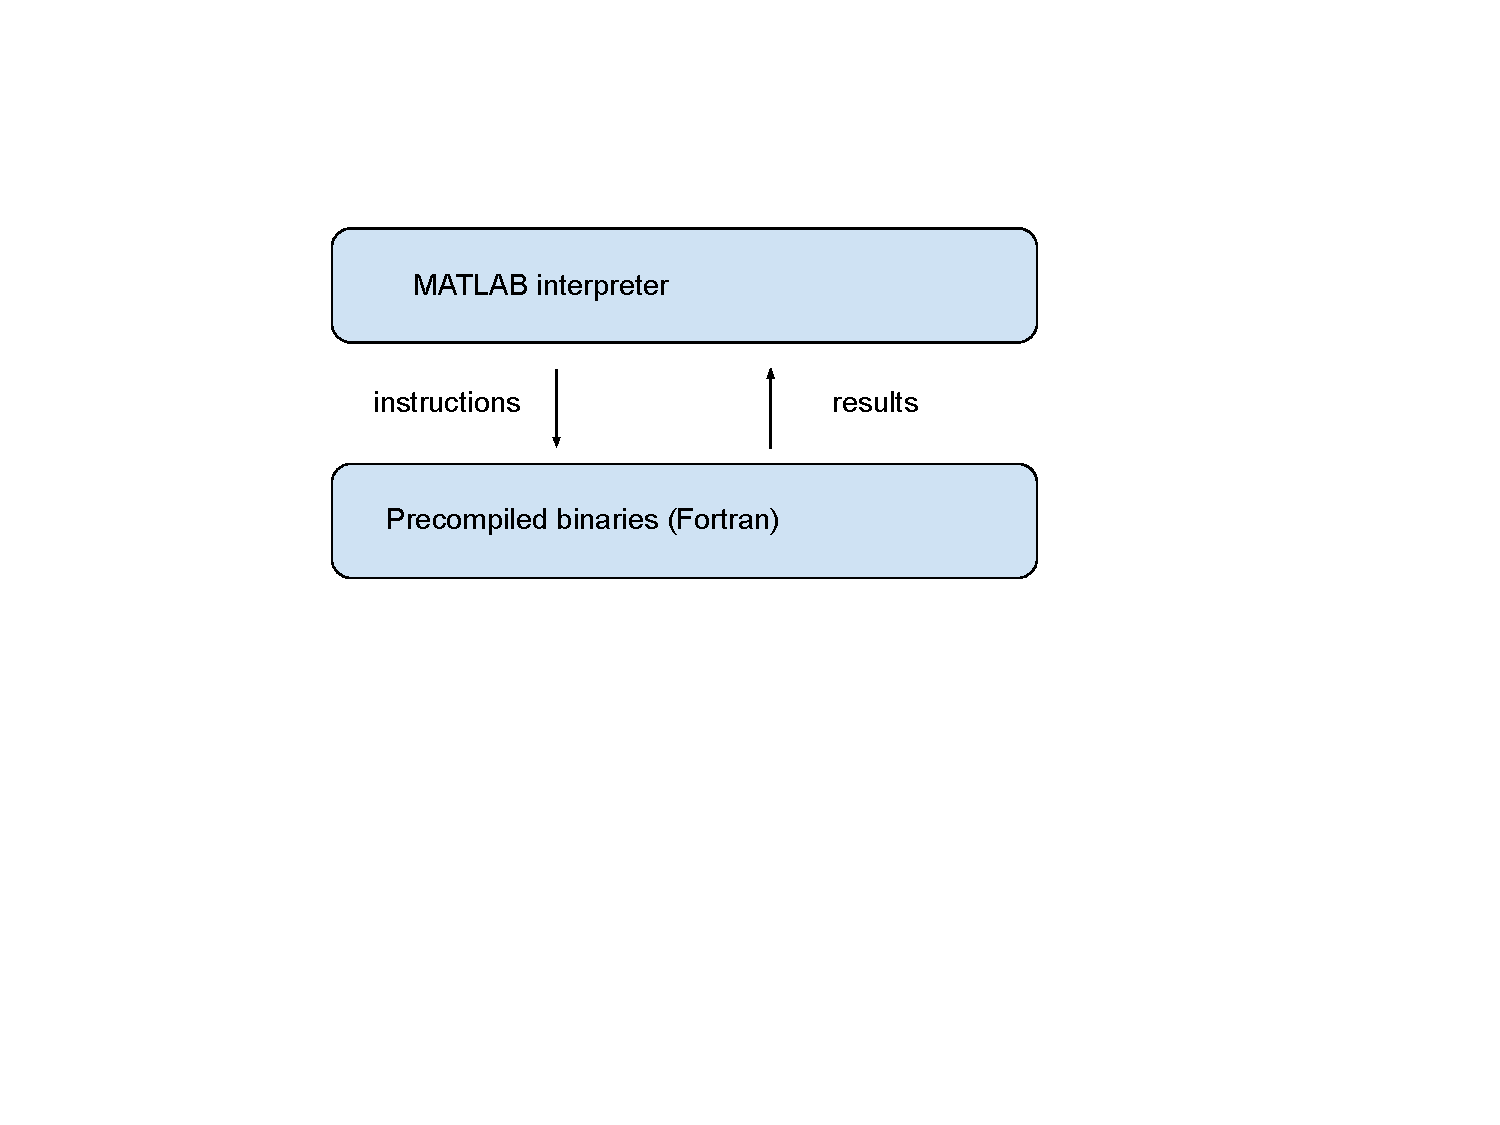
\includegraphics[trim={2cm 8cm 6cm 3cm},clip]{matlab.pdf}}
       \end{center}
    \end{figure}

    
\end{frame}


\begin{frame}
    \frametitle{Python + NumPy -- stealing MATLAB's idea}

    \begin{figure}
       \begin{center} % l b r t
        \scalebox{.6}{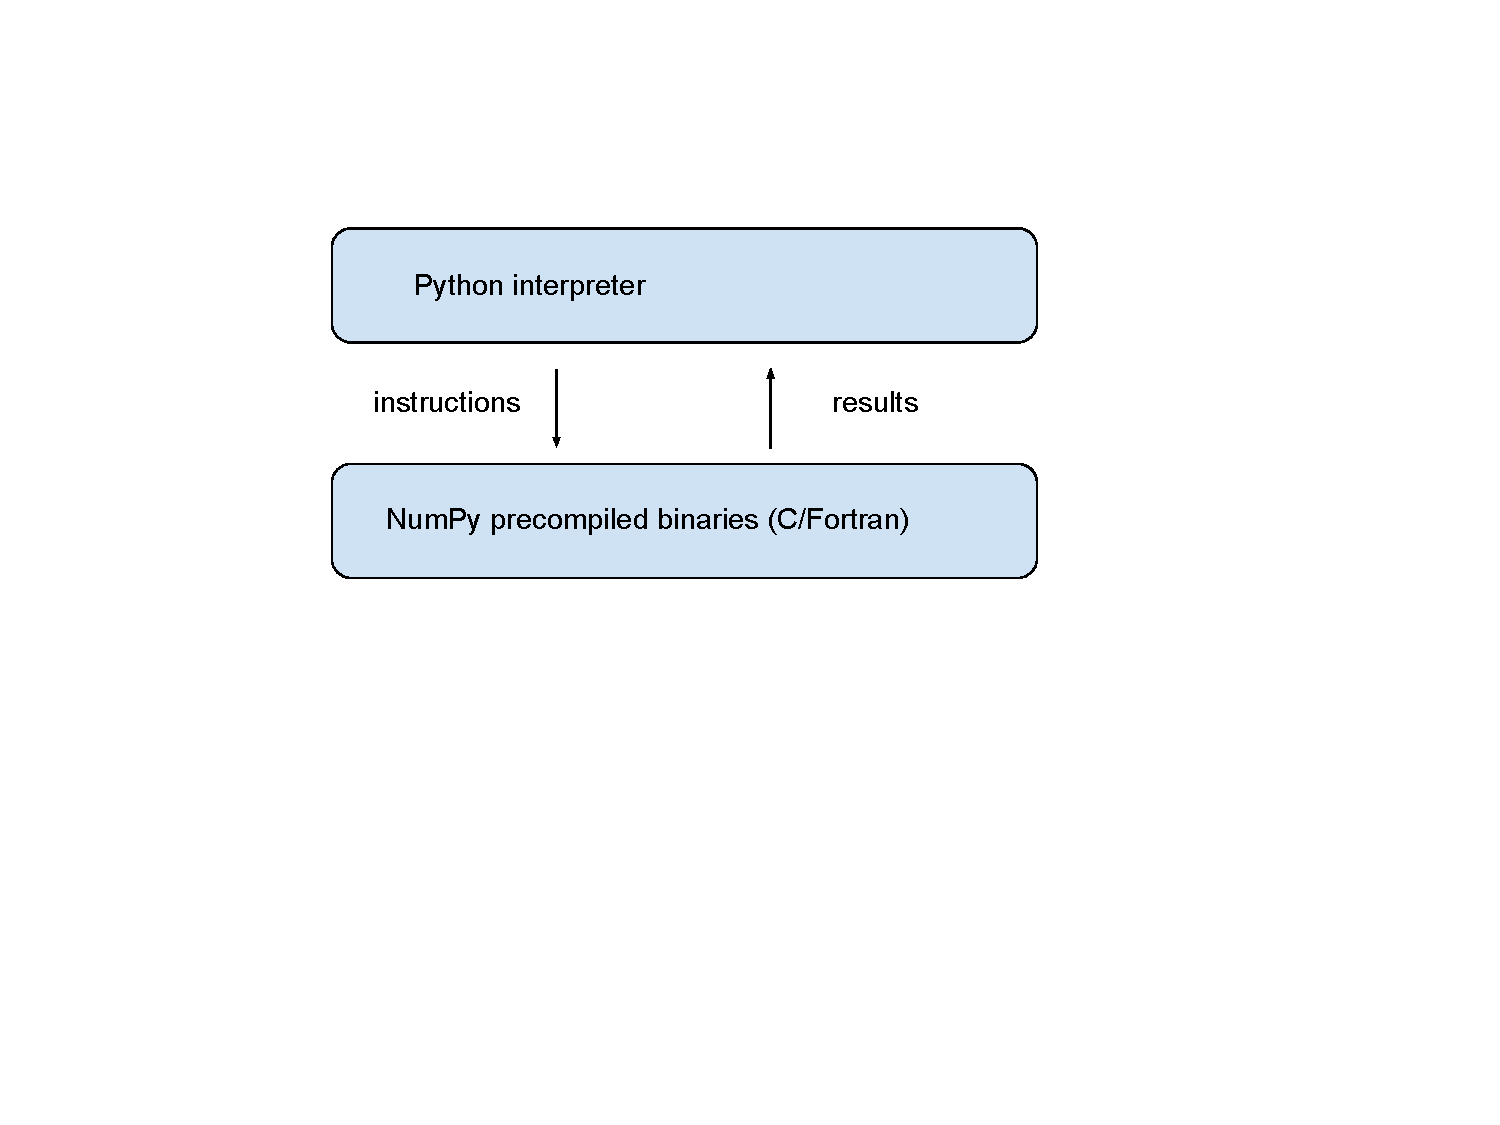
\includegraphics[trim={2cm 8cm 6cm 3cm},clip]{numpy.pdf}}
       \end{center}
    \end{figure}


\end{frame}


\begin{frame}
    \frametitle{Vectorization: pros and cons}

    \navy{Pros}

    \begin{itemize}
        \item fast array operations
        \item high interactivity 
    \end{itemize}

    \vspace{0.5em}
    \vspace{0.5em}

    \navy{Cons}

    \begin{itemize}
        \item some tasks cannot be efficiently vectorized
        \vspace{0.2em}
        \item cannot adapt flexibly to function arguments /
            hardware
    \end{itemize}


\end{frame}




\begin{frame}[fragile]
    \frametitle{Julia --- rise of the JIT compilers}
    
    \begin{minted}{julia}
function solow(k0, α=0.4, δ=0.1, n=1_000)
    k = k0
    for i in 1:(n-1)
        k = s * k^α + (1 - δ) * k
    end
    return k
end

solow(0.2)
    \end{minted}

    Function \texttt{solow} is efficiently JIT compiled after the first call

\end{frame}

\begin{frame}[fragile]
    \frametitle{Python + Numba copy Julia}
    
    \begin{minted}{python}
from numba import jit

@jit
def solow(k0, α=0.4, δ=0.1, n=1_000):
    k = k0
    for i in range(n-1):
        k = s * k**α + (1 - δ) * k
    return k

solow(0.2)
    \end{minted}


    Runs at same speed as Julia / C / Fortran

\end{frame}


\begin{frame}
    
    Notice that most discussion so far is about execution speed on a
    \navy{single} thread...


    \vspace{0.5em}
    \vspace{0.5em}
    \vspace{0.5em}


    Later we'll discuss parallelization

\end{frame}

\begin{frame}

    Some trends: 

    \begin{figure}
       \begin{center}
        \scalebox{0.4}{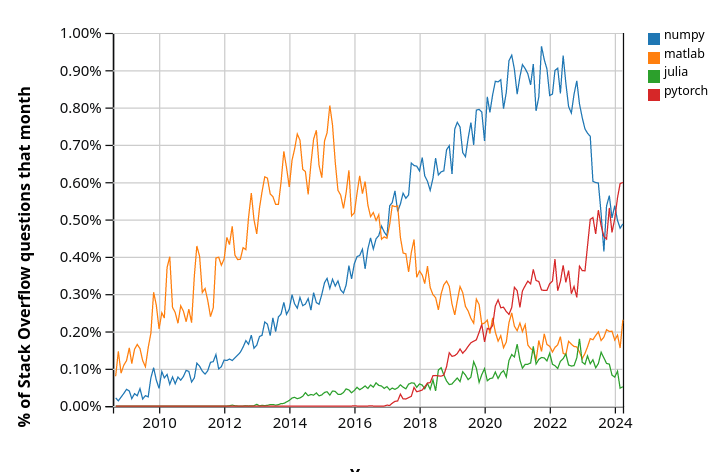
\includegraphics{pvr.png}}
       \end{center}
    \end{figure}

\end{frame}



\begin{frame}
    
    So where does JAX fit in?

        \vspace{0.5em}
        \vspace{0.5em}
        \vspace{0.5em}
        \vspace{0.5em}
        \vspace{0.5em}
    Let's start with some motivation and background

\end{frame}



\begin{frame}
    \frametitle{AI-driven scientific computing}

    AI is changing the world

    \begin{itemize}
        \item image processing / computer vision
        \vspace{0.5em}
        \item speech recognition, translation
        \vspace{0.5em}
        \item forecasting and prediction 
        \vspace{0.5em}
        \item generative AI
    \end{itemize}

    \pause

        \vspace{0.5em}
        \vspace{0.5em}
        \vspace{0.5em}
    Plus killer drones, skynet, etc.\ldots

    
\end{frame}

\begin{frame}
    
    Projected spending on AI in 2024:

    \begin{itemize}
        \item Google: \$48 billion
        \vspace{0.5em}
        \item Microsoft: \$60 billion
        \vspace{0.5em}
        \item Meta: \$40 billion
        \vspace{0.5em}
        \item etc.
    \end{itemize}

\end{frame}



\begin{frame}
    \frametitle{Deep learning in two slides}
    
    We postulate a relationship between inputs and outputs
    %
    \begin{equation*}
        y = f(x)
        \qquad (x \in \RR^k, \; y \in \RR)
    \end{equation*}

    \Egs
    %
    \begin{itemize}
        \item $x = $ sequence of words, $y = $ next word
        \vspace{0.5em}
        \item $x = $ weather sensor data, $y = $ max temp tomorrow
    \end{itemize}
        \vspace{0.5em}
        \vspace{0.5em}

    Problem:

    \begin{itemize}
        \item observe $(x_i, y_i)_{i=1}^n$ and seek $f$ such that $y_{n+1}
            \approx f(x_{n+1})$
    \end{itemize}


\end{frame}


\begin{frame}

    Training: given parametric class $\{f_\theta\}_{\theta \in \Theta}$,
    minimize the loss
    %
    \begin{equation*}
        \ell(\theta) := \sum_{i=1}^n (y_i - f_\theta(x_i))^2
        \quad \st \quad \theta \in \Theta
    \end{equation*}
    %

    \pause
    \vspace{0.5em}
    \vspace{0.5em}
    In the case of ANNs, 
    %
    \begin{equation*}
        f_\theta
        = \sigma \circ A_{1} 
            \circ \cdots \circ \sigma \circ A_{k-1}  \circ \sigma \circ A_{k}
    \end{equation*}
    %
    where
    %
    \begin{itemize}
        \item $A_{i} x = W_i x + b_i $ is an affine map 
        \vspace{0.5em}
        \item $\sigma$ is a nonlinear ``activation'' function
    \end{itemize}

\end{frame}


\begin{frame}
    

    Minimizing a smooth loss functions  -- what algorithm?
    
    \begin{figure}
       \begin{center}
        \scalebox{0.15}{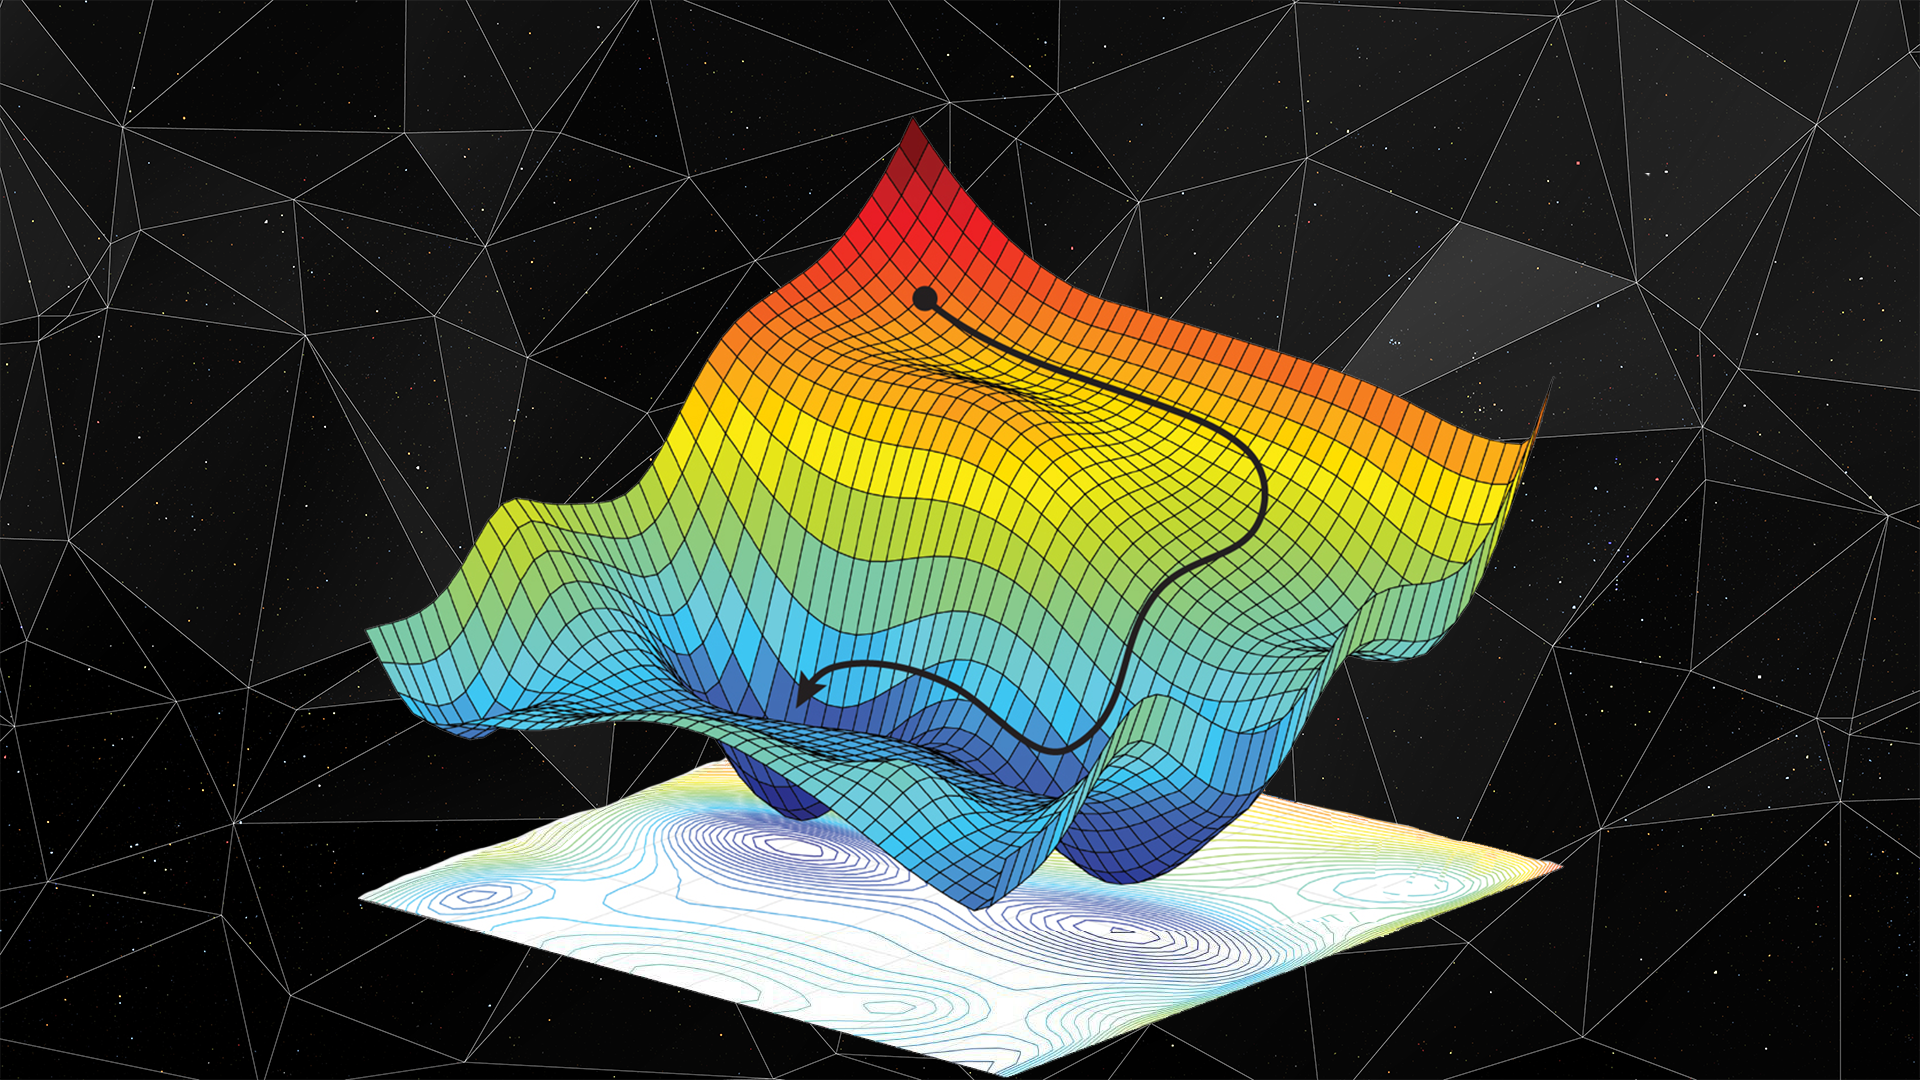
\includegraphics[trim={0cm 0cm 0cm 0cm},clip]{gdi.png}}
       \end{center}
    \end{figure}

    Source: \url{https://danielkhv.com/}

\end{frame}


\begin{frame}

    Deep learning: $\theta \in \RR^d$ where $d = ?$
    
    \begin{figure}
       \begin{center}
        \scalebox{0.14}{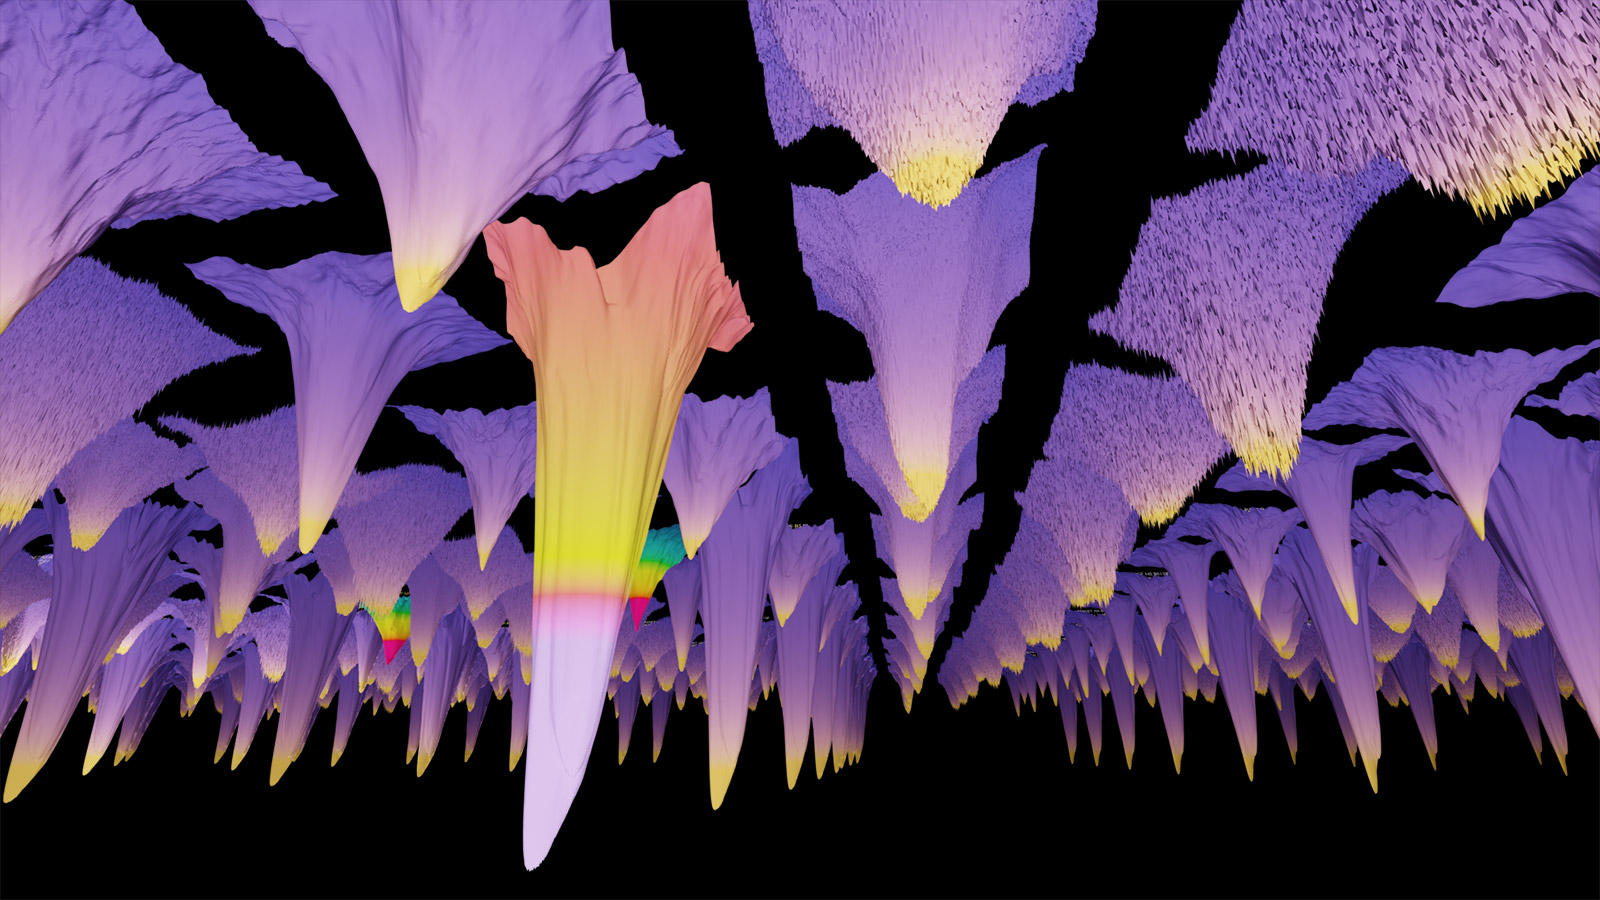
\includegraphics[trim={0cm 0cm 0cm 0cm},clip]{loss2.jpg}}
       \end{center}
    \end{figure}

    Source: \url{https://losslandscape.com/gallery/}

\end{frame}

\begin{frame}
    \frametitle{Hardware}
    
    \begin{figure}
       \begin{center}
        \scalebox{0.18}{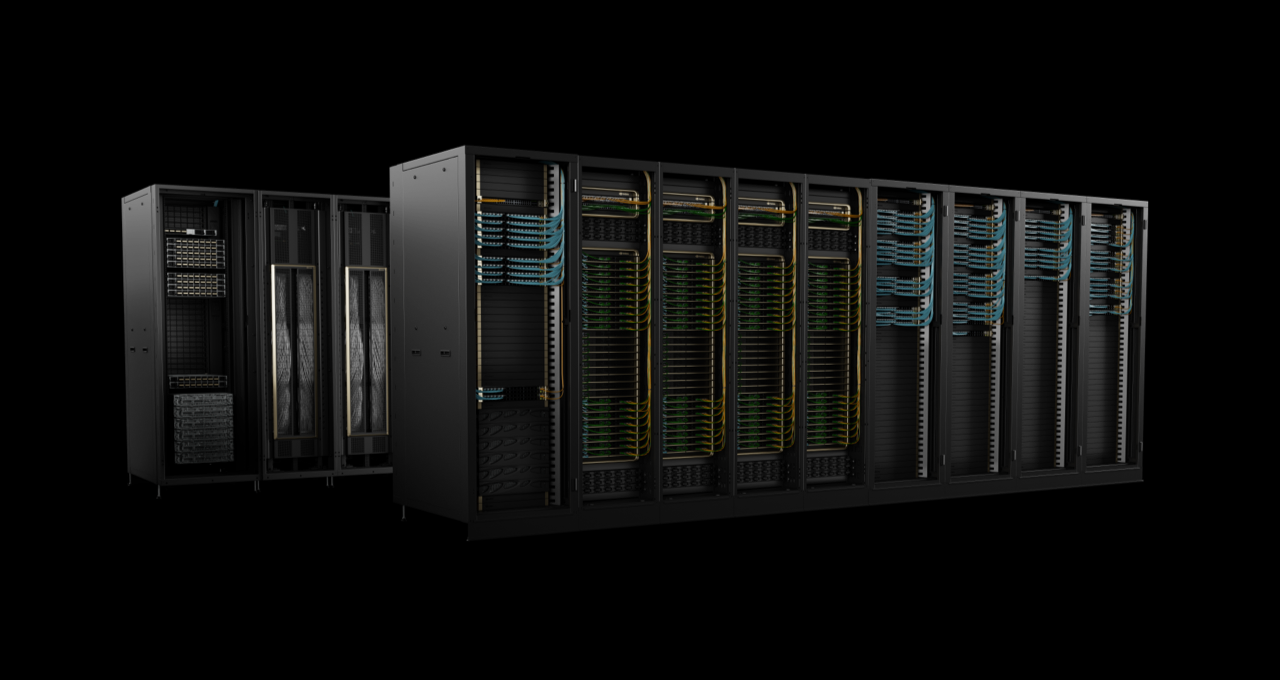
\includegraphics[trim={0cm 0cm 0cm 0cm},clip]{dgx.png}}
       \end{center}
    \end{figure}


\end{frame}


\begin{frame} 
    
    ``NVIDIA supercomputers are the factories of the AI industrial
    revolution.'' -- Jensen Huang


    \vspace{1em}
    \vspace{1em}
    \vspace{1em}

    \begin{itemize}
        \item How many GPUs did OpenAI use to train ChatGPT 4?
    \end{itemize}

\end{frame}




\begin{frame}
    \frametitle{Software}
    
    Core elements
    %
    \begin{itemize}
        \item automatic differentiation (for \underline{gradient} descent)
        \vspace{0.5em}
        \vspace{0.5em}
        \item parallelization --- exploit parallel hardware!
        \vspace{0.5em}
        \vspace{0.5em}
        \item Compilers / JIT-compilers
    \end{itemize}

    \pause
        \vspace{0.5em}

        \vspace{0.5em}
        \vspace{0.5em}
    Crucially, these components must be \underline{well integrated}

        \vspace{0.5em}
        \vspace{0.5em}

    One library with these features is...


\end{frame}


\begin{frame}
    

    \begin{figure}
       \begin{center}
        \scalebox{2.0}{
\includegraphics[trim={0cm 0cm 0cm 0cm},clip]{jax.png}}
       \end{center}
    \end{figure}


\end{frame}


\begin{frame}[fragile]
    
    \vspace{-1em}
    \begin{minted}{python}
import jax.numpy as jnp
from jax import grad, jit

def f(θ, x):
  for W, b in θ:
    w = W @ x + b
    x = jnp.tanh(w)  
  return x

def loss(θ, x, y):
  return jnp.sum((y - f(θ, x))**2)

grad_loss = jit(grad(loss))  # Now use gradient descent 
    \end{minted}

    {\footnotesize Source: JAX readthedocs}

\end{frame}



\begin{frame}
    \frametitle{JAX for economists}

    JAX is obviously useful if you do deep learning
    \vspace{0.5em}
    \vspace{0.5em}

    But what about \underline{me}?

    \vspace{0.5em}
    \vspace{0.5em}
    \vspace{0.5em}
    I do mathematical modeling / optimization / simulation
    

\end{frame}



\begin{frame}
    

    My wishlist:

    \begin{itemize}
        \item exposes low level operations 
        \vspace{0.5em}
        \item \underline{automated} parallelization
        \vspace{0.5em}
        \item JIT compiler 
        \vspace{0.5em}
        \item integrated autodiff
        \vspace{0.5em}
        \item \underline{automatically} / transparently supports CPUs / GPUs / TPUs 
    \end{itemize}

    \vspace{0.5em}
    \vspace{0.5em}
    JAX ticks these boxes



\end{frame}

\begin{frame}
    

    Comments:

    \begin{itemize}
        \item JAX is not an open source project in the same sense as Julia or NumPy!
        \vspace{0.5em}
        \item JAX wants vectorized code, not loops
    \end{itemize}

        \vspace{0.5em}
        \vspace{0.5em}
        \vspace{0.5em}

    Reminders:

    \begin{itemize}
        \item Please stick around for a photo at the end
        \vspace{0.5em}
        \item I'm on the road next year in case there's demand for workshops
    \end{itemize}


\end{frame}



\end{document}


